\documentclass[10pt]{beamer}

\usetheme{metropolis}
%\usecolortheme{owl} % dark theme
%\usecolortheme[snowy]{owl} % black on white
\usepackage{appendixnumberbeamer}
\usepackage[T1]{fontenc}
\usepackage[utf8]{inputenc}
% \usepackage{lmodern}
\usepackage{tikz}   

\usepackage{booktabs}
\usepackage[scale=2]{ccicons}

\usepackage{pgfplots}
\usepgfplotslibrary{dateplot}

\usepackage{xspace}
\usepackage{tabularx}

\newcommand{\themename}{\textbf{\textsc{metropolis}}\xspace}

\title{HOOT Augmented reality ads- Hoot AR revenue strategy}
\subtitle{Performant AR ads with measurable ROI  - making video ads perform using augmented reality}
\date{\today}
\author{Hoot Ar ads team}
\institute{Hoot Live inc., a Delaware C-corp}
% \titlegraphic{\hfill
\includegraphics[height=1.5cm]{logo.pdf}}

\begin{document}

\maketitle

% \begin{frame}{Table of contents}
%   \setbeamertemplate{section in toc}[sections numbered]
%   \tableofcontents[hideallsubsections]
% \end{frame}

% \section{Primer}

\begin{frame}[fragile]{Current landscape in digital video advertising }

\begin{itemize}
\item[-]business model for video advertising is CPM (cost per million impressions) which doesn’t provide accurate ROI for advert buyers
  
\item[-]Many ad-bots end up generating fake views of the video ad creating uncertainty and speculation about the ad’s effectiveness and ROI
\item[-]Viewers aren’t engaged enough in the ad leading to sales causing major drop off for advertisers
Hoot Network acts as a marketplace, its Open Source software allows anyone to join the network both 
\end{itemize}

\end{frame}
\begin{frame}[t]{Problems of current model}
\begin{itemize}
\item[-]No clear call to actions in video ads
\item[-]Viewers confused as to what to do after watching video
\item[-]Unclear ROI to advertisers
\end{itemize}

Video ads are stuck in the banner ad dark ages pre-Google adwords 

\end{frame}
\begin{frame}[t]{Hoot Augmented Reality ads }
\begin{itemize}
\item[*]Augmented reality ads create great engagement with users in key ways
\item[*]Personalization, users can upload photos of themselves and become part of the ad ie their  bitmoji AR avatars (masquerade) 
\item[*]Content and Virality: celebrities like Rihanna can increase engagement by her presence in an AR ad and can go viral given her popularity
\item[*]Calls to action: Buy now buttons can be added to the ad, Buy concert ticket to Rihanna event
\end{itemize}
\end{frame}
%--- Next Frame ---%


\begin{frame}[fragile]{Solutions - Building Adwords of video}
\begin{itemize}
\item[+]Clear and engaging call to actions in video ads using AR
\item[+]Viewers know what to do after watching video by clicking call to action buy 
\item[+]Clear AR ad performance ROI to advertisers 

Hoot AR ads helps usher a golden age of performant video ads like Google adwords did to banner ads

\end{itemize}


\end{frame}
\begin{frame}[t]{CPR model - video adwords}
\begin{itemize}
\item[*]CPR model using Vickrey auctions allows Hoot to monetize only if the consumer clicks through to advertisers call to action ie charge based on a CPR model cost per referral
\item[*]This benefits advertisers so they can see clear ROI Referrals > Impressions
\item[*]This benefits hoot as we can charge based on effectiveness as Google adwords is able to charge more based on performance laying foundations for a billion dollar ad business
\end{itemize}
\end{frame}
\begin{frame}[standout]
  Hoot AR ads Questions? - building Adwords of the web
  \begin{tikzpicture}
  \node (img1) {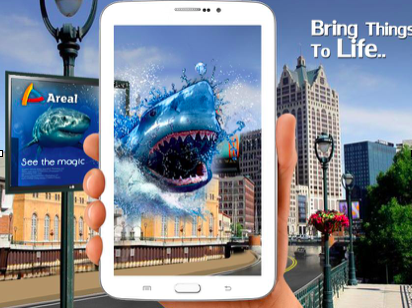
\includegraphics[height=5cm]{static/arad/arad1}};
  % \pause
  \node (img2) at (img1.south east) [xshift=-1cm] {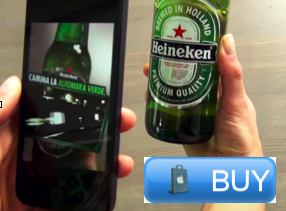
\includegraphics[height=4cm]{static/arad/arad3}};
  % \pause
  \node (img3) at (img2.south west) [xshift=-2cm,yshift=1cm] {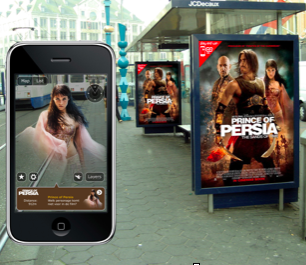
\includegraphics[height=4cm]{static/arad/arad2}};
  \pause
  \node (img4) {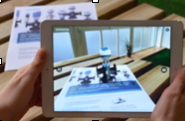
\includegraphics[height=5cm]{static/arad/arad4}};
  % \pause
  \node (img5) at (img1.south east) [yshift=-1cm] {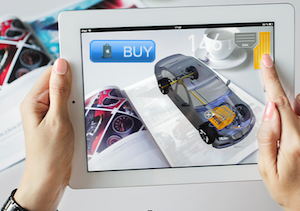
\includegraphics[height=4cm]{static/arad/arad5}};
  
  \end{tikzpicture}
  
\end{frame}


\end{document}
